\chapter{Estratégias de Abordagem aos Problemas} \label{cap:abordagem}
Neste capítulo vamos analisar os procedimentos, tecnologias e conceitos utilizados no desenvolvimento deste projeto. Na secção \ref{sec:dados} propomos um modelo para a estrutura de dados utilizada neste sistema. Na secção \ref{sec:ecra} vamos apresentar esboços para os ecrãs da aplicação para os utilizadores.

%MODELO DE DADOS ......................................................................................
\section{Modelo de Dados} \label{sec:dados}
Um dos componentes deste sistema é um repositório de dados, que irá conter as várias informações relacionadas com os clientes deste serviço. Na figura \ref{fig:relacoes} está representado de forma gráfica o modelo dos dados guardados neste repositório. \\

\begin{figure}[ht!]
\centering
\resizebox{90mm}{!}{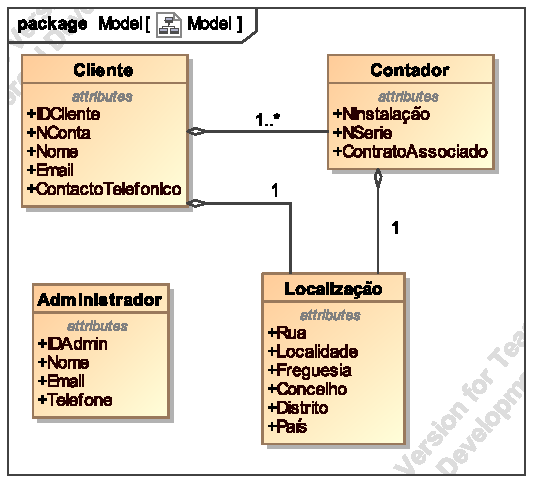
\includegraphics{diagramas/svg/uml__Model.pdf}}
\caption{Arquitetura do sistema.}
\label{fig:relacoes}
\end{figure}

O elemento cliente representa um cliente do serviço que utiliza o sistema. Para cada cliente será registado um ID único  \texttt{(IDCliente)}, o seu \texttt{nome}, \texttt{email}, número de telefone/telemóvel (\texttt{Telefone}) e \texttt{número de conta}. \\
Também existem utilizadores com papel de administrador, para os quais registamos um ID único (\texttt{IDAdmin}), o seu \texttt{nome}, \texttt{email} e número de telefone/telemóvel(\texttt{Telefone}) . \\
Os clientes terão associado um ou mais contadores, pelo que para cada contador guardamos o seu número único de instalação (\texttt{NInstalação}), o seu número de série (\texttt{NSerie}) e o contrato (\texttt{ContratoAssociado}) e o cliente (\texttt{IDCliente}) aos quais este contador está associado. \\
Cada contador tem uma localização, que representa o local onde o contador está instalado. Cada cliente tem também uma localização associada, que representa a sua morada principal para onde é, por exemplo, enviado o correio postal. Uma localização segue a estrutura normal de uma morada: \texttt{rua}, \texttt{localidade}, \texttt{freguesia}, \texttt{concelho}, \texttt{distrito} e \texttt{país}.

%ECRAS ...........................................................................................................
\section{Ecrãs da Aplicação Móvel} \label{sec:ecra}
Nesta secção apresentamos os vários esboços que desenhámos para os ecrãs ou páginas da aplicação móvel.\\
Na figura \ref{fig:1} está a página de \textit{log-in}.

\begin{figure}[ht!]
\centering
\resizebox{40mm}{!}{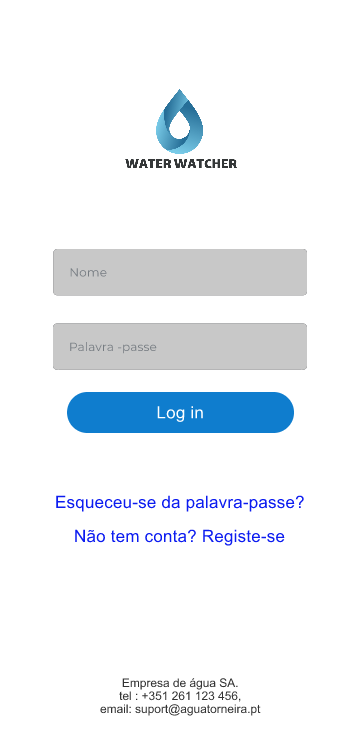
\includegraphics{diagramas/app/1.png}}
\caption{Página de log-in.}
\label{fig:1}
\end{figure}

Nesta página é possível o utilizador inserir as suas credenciais para entrar na aplicação. Também é possível registar uma nova conta ou recuperar o acesso a uma conta. Esta página apresenta também os contactos da empresa.\\
Depois de efetuado o \textit{log-in}, o utilizador é encaminhado para a página principal, apresentada na figura \ref{fig:2}.

\begin{figure}[ht!]
\centering
\resizebox{40mm}{!}{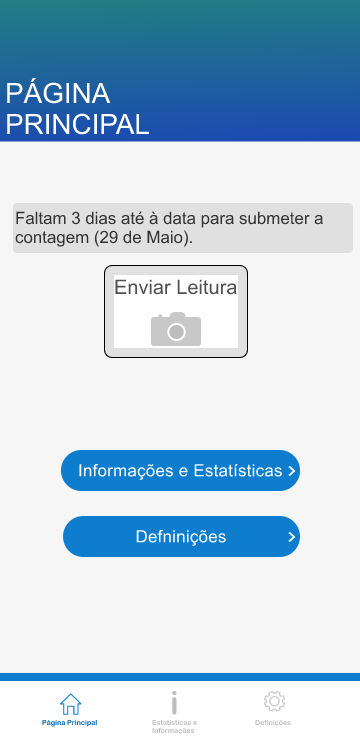
\includegraphics{diagramas/app/2.png}}
\caption{Página principal}
\label{fig:2}
\end{figure}

É neste ecrã que o utilizador poderá enviar a fotografia do contador no dia designado. \\
A partir deste ecrã, tem também a possibilidade de aceder às informações e estatísticas presentes no ecrã representado na figura \ref{fig:3}. 

%\vspace{8.5cm}

\begin{figure}[ht!]
\centering
\resizebox{40mm}{!}{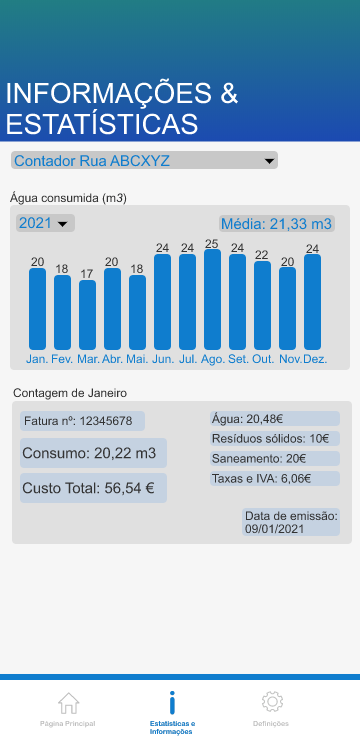
\includegraphics{diagramas/app/3.png}}
\caption{Página de informações e estatísticas}
\label{fig:3}
\end{figure}

A página de informações e estatísticas é onde estão disponíveis vários dados referentes ao serviço e detalhes das faturas do utilizador.\\ 
Por fim, é possível aceder ao ecrã de definições representado na figura \ref{fig:4}.

\vspace{1cm}

\begin{figure}
\centering
\begin{minipage}{.5\textwidth}
 \centering
\resizebox{40mm}{!}{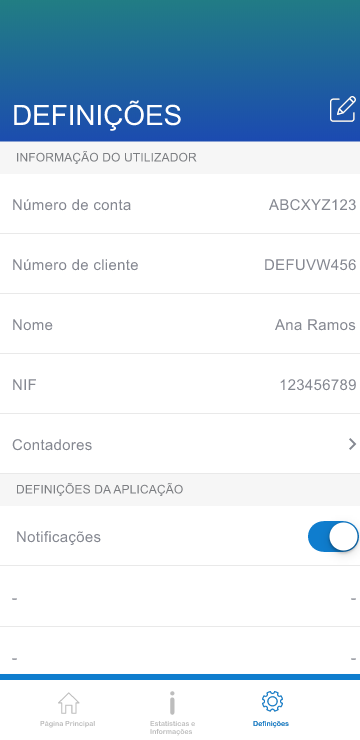
\includegraphics{diagramas/app/4.png}}
\caption{Página de definições.}
\label{fig:4}
\end{minipage}%
\begin{minipage}{.5\textwidth}
  \centering
\resizebox{40mm}{!}{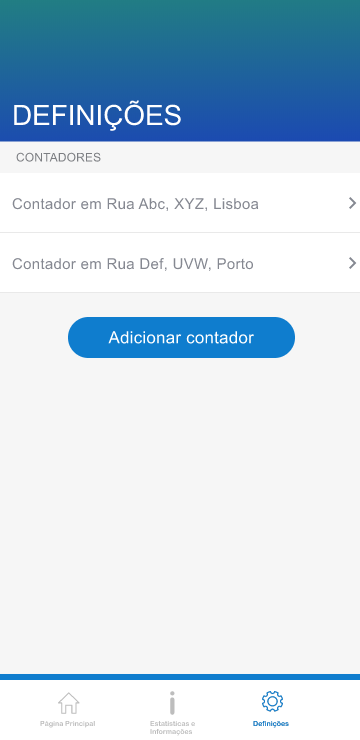
\includegraphics{diagramas/app/5.png}}
\caption{Página de definições relacionadas com os contadores.}
\label{fig:5}
\end{minipage}
\end{figure}

Nesta página, o utilizador pode ver e editar as suas informações e preferências da aplicação. Mais concretamente, também é possível gerir os contadores associados à sua conta, no ecrã da figura \ref{fig:5}.

\section{Reconhecimento de Caracteres} \label{caracteres}
Este sistema vai reconhecer caracteres presentes nas fotografias dos contadores dos clientes. Para melhorar a qualidade e eficácia do reconhecimento de caracteres decidimos estudar e testar vários tipos de imagens de um contador para perceber em quais é que o reconhecimento de caracteres era mais eficaz.
Para este teste utilizamos as seguintes imagens:\\
\par1-Imagem digital de números pretos em fundo branco, de referência.
\par2-Fotografia do contador.
\par3-Fotografia do contador cortada de forma a só conter o mostrador dos números.
\par4-Fotografia 3 em preto e branco.
\par5-Fotografia 3 com as cores invertidas.
\par6-Fotografia 3 com as dimensões aumentadas.\\

Obtivemos mais sucesso, ou seja, o texto obtido através do reconhecimento de caracteres ser mais próximo dos números reais presentes no contador, com a fotografia restringida ao mostrador do contador com as cores invertidas.

\section{Programa de Controlo Semanal} \label{rec}
Existirá uma forma de os clientes do serviço poderem ter um maior controlo do seu consumo de água, nomeadamente, saber o seu gasto em períodos menores do que mensalmente.\\
Propomos a implementação de um processo, totalmente opcional e que não interfere com a restante utilização do sistema, que lembra os utilizadores semanalmente de enviar a contagem do seu contador.\\
Estes envios terão como propósito poder apresentar ao utilizador o seu gasto de água semanal, permitindo que este, por exemplo, alterando os seus hábitos de consumo de água, consiga observar alterações mais imediatas nas suas contagens. Por outro lado, a empresa terá também acesso a estas contagens.\\
Estas contagens têm uma função meramente informativa e são de carater opcional.


\section{Biblioteca de Reconhecimento de Caracteres} \label{rec}
Para o reconhecimento de caracteres elaborámos uma extensão Outsystems que tem por base a biblioteca Tesseract \cite{tesseract}.\\
A biblioteca Tesseract é uma biblioteca open source muito utilizada no reconhecimento de caracteres em imagem por ser facilmente configurável consoante a linguagem ou tipo de caracteres que se pretende extrair. Implementa uma rede neuronal para a deteção dos caracteres e utiliza um ficheiro de configuração configurado para detetar dígitos presente em \ref{tes:digits}.


















